\begin{figure*}
  \vspace{-1.5em}
  \centering
  \updatedFigure{
    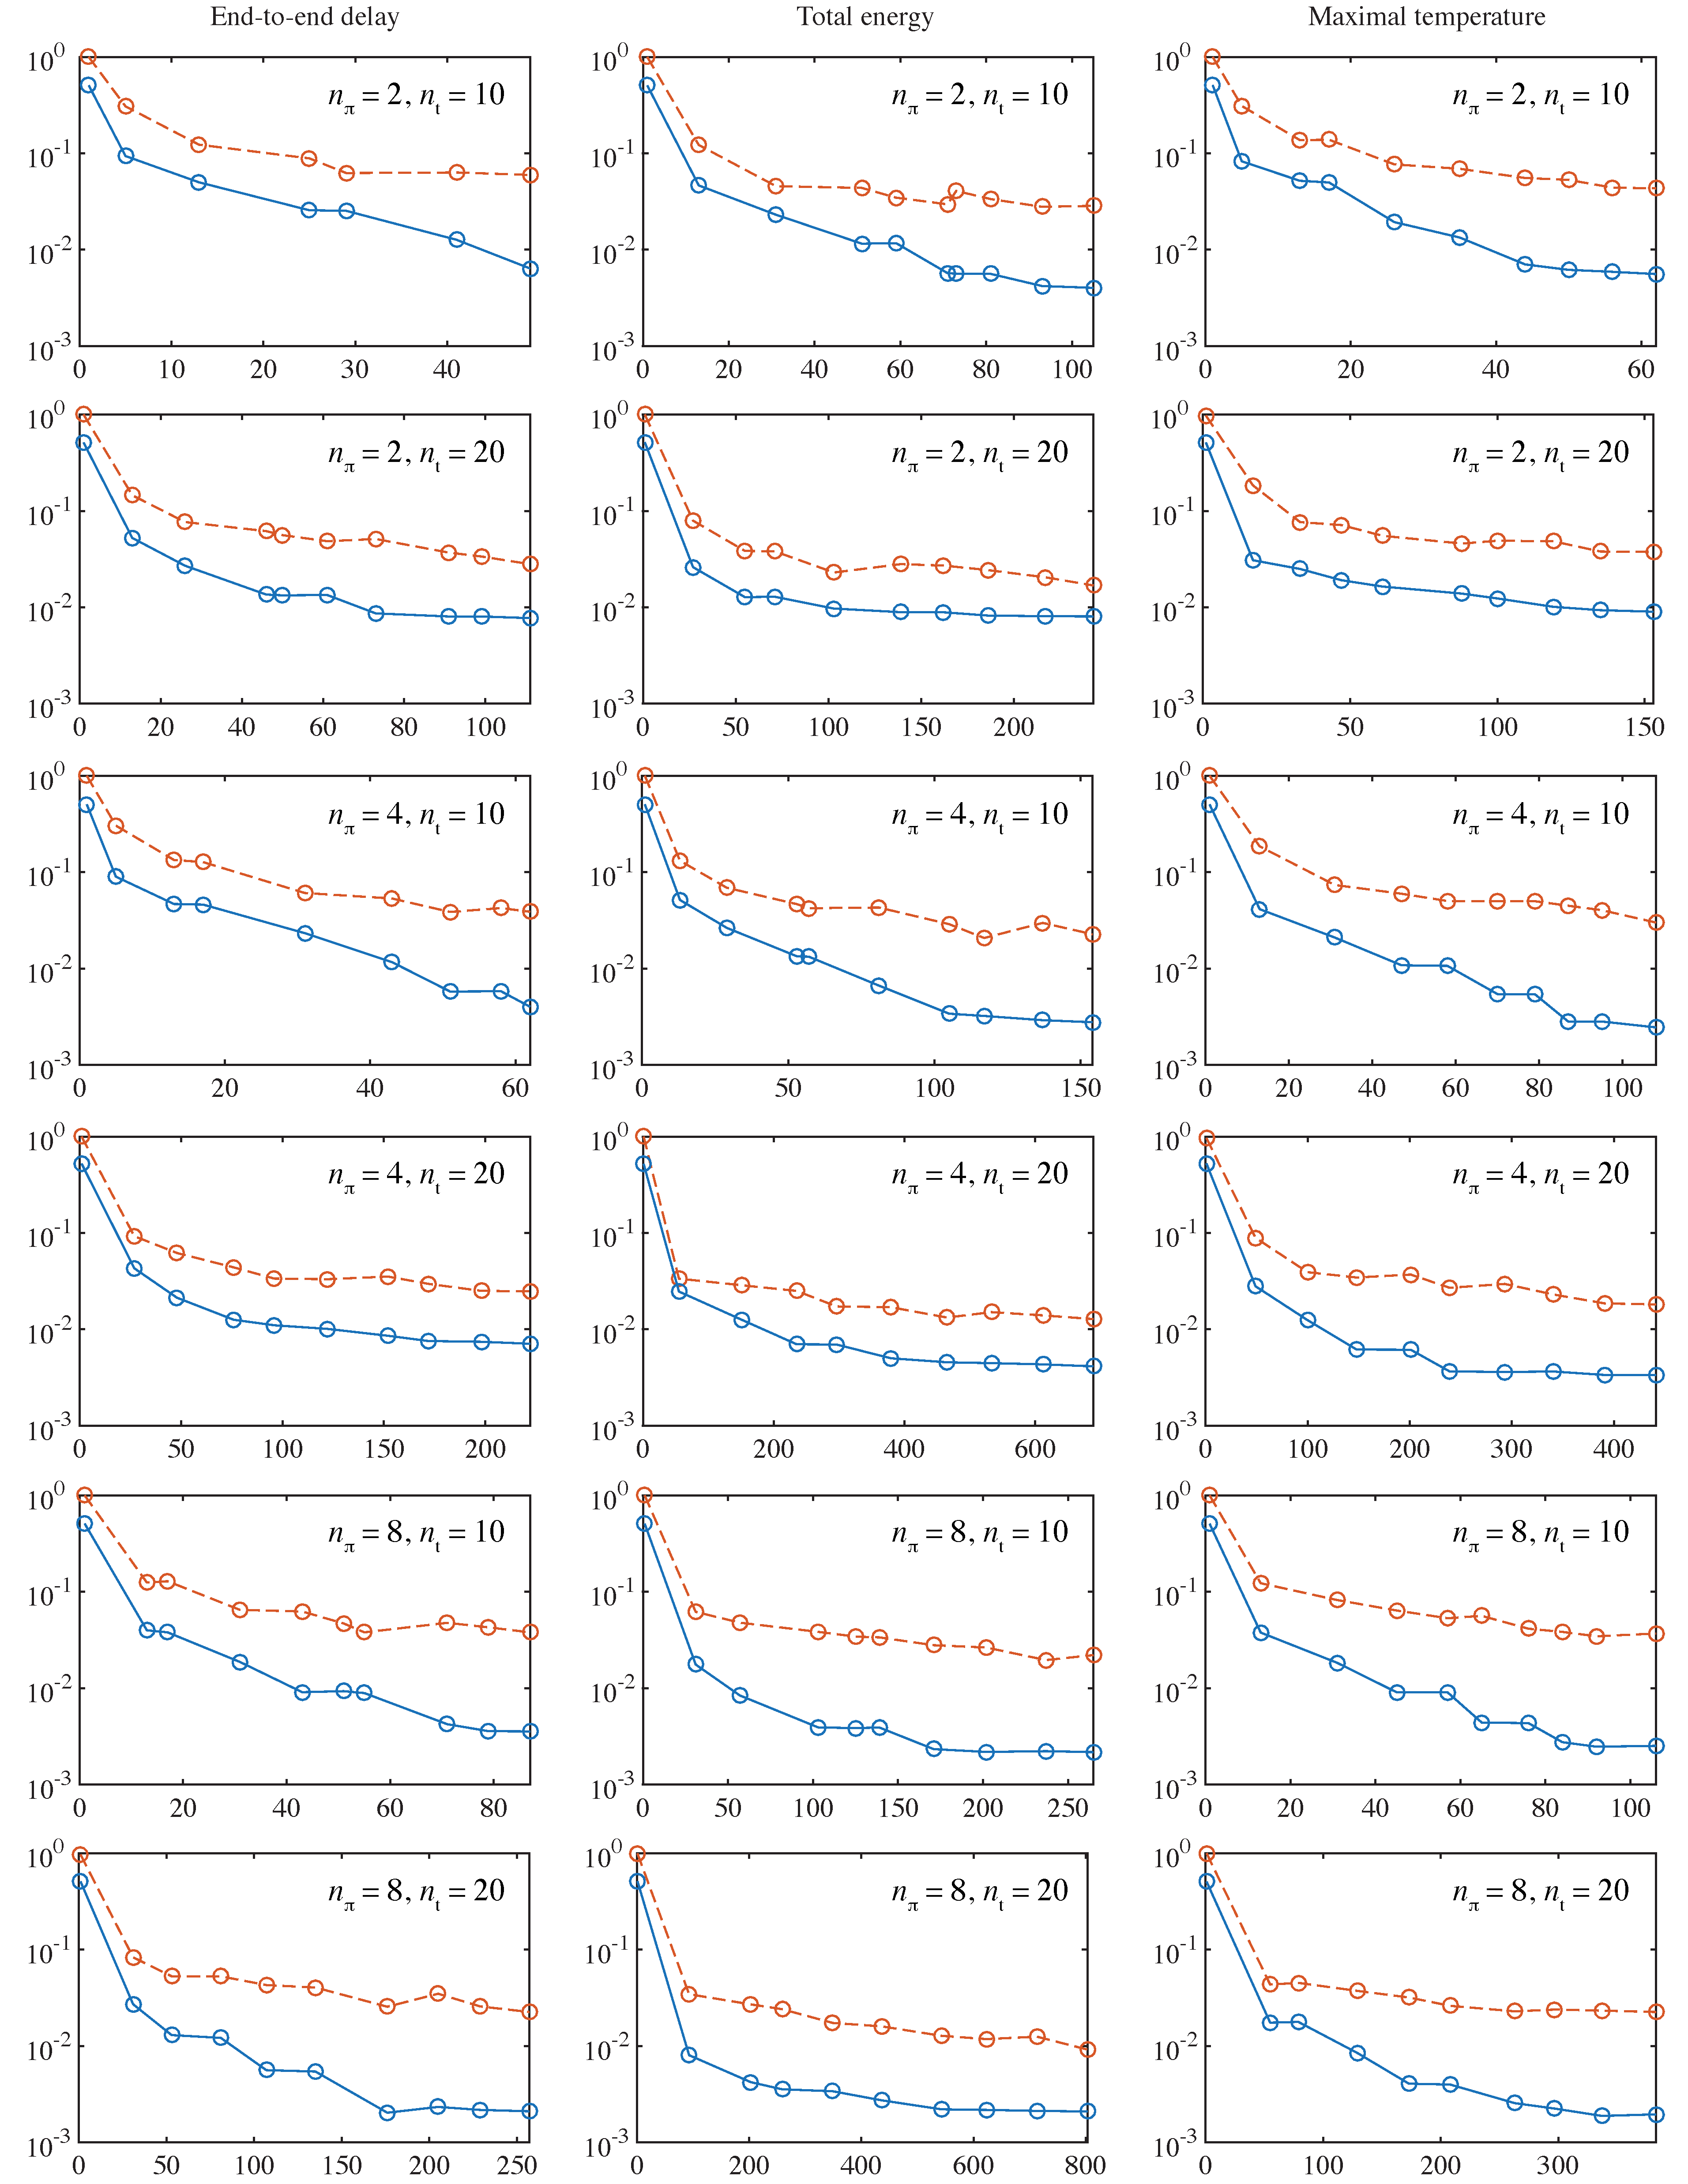
\includegraphics[width=1.0\textwidth]{include/assets/figures/results.pdf}
  }
  \vspace{-1.5em}
  \caption{
    Experimental results. \updated{The columns correspond to the metrics written
    at the very top.} The horizontal axes show the number of points, and the
    vertical ones the error on logarithmic scales. The solid lines correspond to
    the proposed technique, and the dashed ones to direct sampling.
  }
  \flab{results}
\end{figure*}
